\documentclass[rapport.tex]{subfiles}

\begin{document}
\section{Implementering}
	\subsection{Indledning}
	\subsection{Bruger-interface og applikation}
	I følgende afsnit vil implementeringen af bruger-interfacet og applikationen blive beskrevet. 
	\subsubsection{UserInterface}
	Biblioteker værd at nævne: Tkinter, Tkfiledialog\\
	
	\begin{figure}
	\centering
	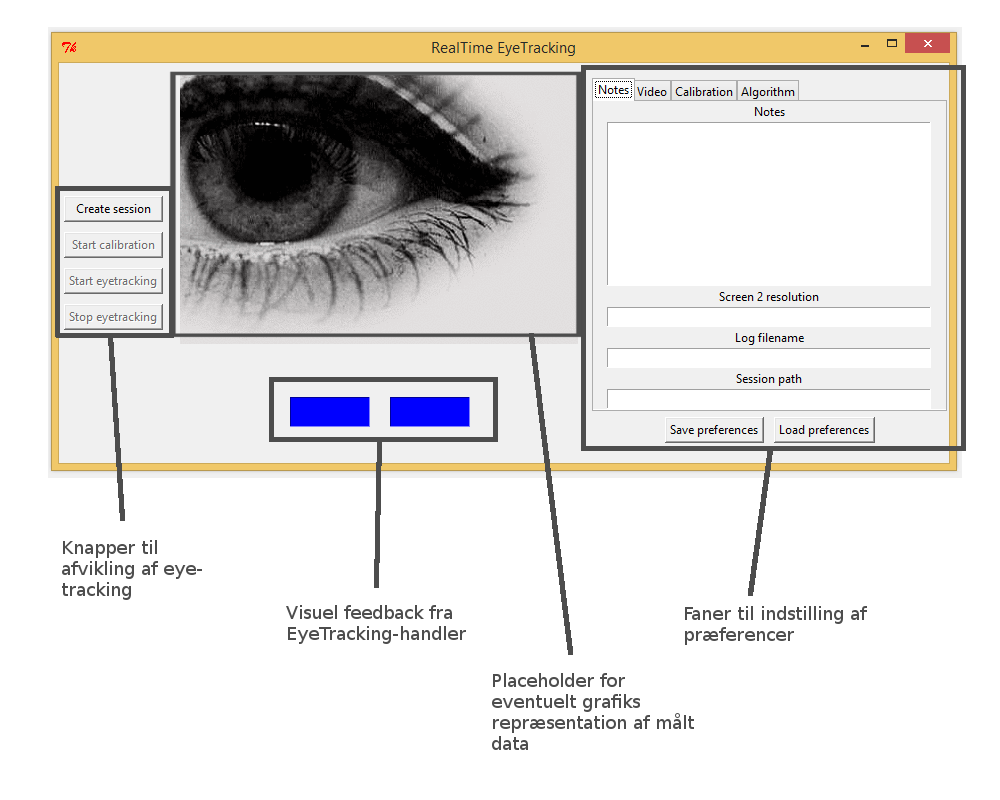
\includegraphics[width=0.9\linewidth]{GUIkommentare}
	\caption[Implementering af GUI]{Implementeringen af det grafiske user-interface med kommentarer}
	\label{fig:GUIkommentare}
	\end{figure}
	
	Tkinter objekter er benyttet til at opbygge det grafisk brugerinterface som givet i design. 
	Hver knap er blevet oprettet med et tilknyttet funktionskald der udfører den ønskede funktion, som givet af de forskellige use cases. 
	Brugeren ser kun Tkinter objekter. 
	Knapperne til venstre i interfacet er sat i rækkefølge efter naturlig opsætning og eksekvering af real-time eye-tracking. Ikke tilgængelige funktioner har deaktiverede knapper således at man ikke kan foretage ulovlige handlinger. \\
	
	De fire faner til højre er til indstilling af præferencer. Herfra kan man tilgå, læse og ændre alle præferencer, samt gemme og indlæse præference-filer.\\
	
	I bunden af bruger-interfacet er to farvede bokse. Disse bokse bruges til at give visuelt feedback bestemt af klassen EyeTrackingHandler. Farven blå indikerer at der ikke kører nogen eye-tracking. Grøn indikerer at eye-tracking kører. Igennem EyeTrackingHandler er det muligt at sætte farven på de to bokse til rød, hvilket kan bruges til at indikere eventuelle fejl. I denne implementering med Starburst-algoritmen er hver boks sat til at repræsentere et øje, således at rød farve indikerer at algoritmen ikke kan finde det tilsvarende øje. 
	Interaktion med andre klasser:
	For hver tilgang til præference-filen bliver der oprettet en ny instans af dataklassen SessionData fra klassen SessionHandler. Ved at aflæse indholdet/værdien af de forskellige Tkiner-objekter og skrive dette data til den instansen af SessionData, der senere bliver skrevet til præference-filen af klassen SessionHandler, vil der altid være konsistens mellem værdierne skrevet i brugerinterfacet, værdierne i præference-filen, og værdierne brugt i eye-tracking-algoritmen. 
	
	
	\subsubsection{SessionHandler}
	SessionHandlers opgave er at stille et data-format til rådighed for kommunikation af sessions-indstillinger de forskellige klasser imellem. Klassens vigtigste opgave er derfor at opretholde et korrekt format. Ved oprettelse eller opdatering af præference-fil, kreerer SessionHandler en streng med henholdsvis navn på variabeltype, variable værdi konverteret til streng (hvis variablen er tom, skrives strengen "None"), efterfulgt af et linebreak. Når strengen er oprettet for alle variabler, skrives strengen til en præference-fil med suffiks .pref. \\
	Når en præference-fil indlæses, verificeres den først af SessionHandler ved at lede efter alle variablenavne i den læste fil. Herefter kan hver variabel udtrækkes fra filen. Det er nødvendigt at lave tjek på hver variabel, da konvertering fra python- og numpy-værdi til streng kan medføre komplikationer. 
	ÆNDRE KODEN SÅLEDES AT SESSIONHANDLER FORETAGER RSTRIP OG SÅ VIDERE 
	
	Figur \ref{list:sessionfile} er et eksempel på præference-fil med korrekt format (Værdierne variablenames og variablevalues er trunkeret for formateringens skyld). 
\begin{figure}
\caption{Eksempel på præference-fil}
\label{list:sessionfile}
\begin{lstlisting}
SESSIONPATH C:/RealTimeEyeTracking
USINGCAM True
CAMNR None
VIDEOPATH 0
NOTES Dette er en testsession
RESOLUTION 1600x900
CALTYPE Numbers
LOGFILENAME testlog
CALFILENAME testcallog
LOADEDCALDATA None
RECORDVIDEO False
RAWDATAPATH None
VARIABLENAMES['e_center', 'last_eyes', ...
VARIABLEVALUES['[0,0]', '[]', 'True', '20', '1500', ...
\end{lstlisting}
\end{figure}
		
	\subsubsection{LogHandler}
	At nævne: StartTracking kører igennem her. Holder værdi om hvorvidt algoritmen kører. Bliver brugt som dataklasse. 
	Modtager en log-streng fra EyeTrackingHandler og gemmer den som angivet i SessionData dataklassen. 
	Vis eksempel på log-fil
	
	\subsubsection{CalibrationHandler}
	Vis eksempel på kalibrerings-fil
	
	\subsubsection{EyeTrackingHandler}
	
	
	\subsubsection{VideoCapture}
	Indeholder puplic funktion GetCameraInputs. 
	Andre funktioner er en del af klassen. Klassen oprettes med et video-input, og mulighed for kalibreringsdataet, samt ti frie variabler. Kalibreringsdataet og de ti frie variabler benyttes ikke til andet end at videresende til ETAlgorithm sammen med gyldig frame. 
	At passe kalibreringsdataet og de frie variabler igennem VideoCapture er ikke optimalt, men spiller ingen rolle i det samlede arbejdslæs. Det kan forestilles at man i stedet ville sende to pointers til hvor disse data ville være lageret. Argumentet for at passe disse data igennem VideoCapture er, at VideoCapture så vil kalde ETAlgorithm's Track() med den fundne frame samt disse data, i stedet for at returnere den fundne frame til EyeTrackingHandler og derefter kalde Track(). 
		
	\subsection{ETAlgorithm}
	Koden i figur \ref{list:emptyalg} er en tom udgave af klassen ETAlgorithm med de nødvendige input-argumenter og funktionskald til EyeTrackingHandler er implementeret:

\begin{figure}
	\caption{Tom udgave af klassen ETAlgorithm}
	\label{list:emptyalg}
\begin{lstlisting}
import numpy as np
import EyeTracking as et

#Her tilfoejes diverse python-biblioteker

def Track(frame, calibration_data, variables):

#Egen kode her 

et.PackWithTimestamp(screen_point, trigger_value)
et.LastRunInfo(variables)
return
\end{lstlisting}
\end{figure}

	
	
	Afsnit \ref{StarburstImpl} beskriver implementering af Starburst-algoritmen i ETAlgorithm.
	\subsection{Starburst-algoritmen}
	\label{StarburstImpl}
	\subsection{Optimering}
	
	\subsubsection{Fremtidige optimeringsmuligheder}
	Python understøtter multitrådning, hvilket giver mulighed for at køre flere instanser af eye-tracking-algoritmen sideløbende. Skriv mere om muligheder for multitrådning, og hvorfor det kan virke.
	\subsection{Diskussion}
		
\end{document}